As a preface to the following numerical validation, it should be mentioned that each of the test cases consist of two-dimensional rectangular domains with no objects in these domains. To be blunt this is a worst case for LABFM, which is a meshless method designed for its effectiveness in `interesting' geometries.

\emph{And rectangles are not interesting.}

Having said that, although the computational time may be larger than if, say, a simple centred finite difference method had been used due to the much larger stencil sizes, the use of LABFM here still provides discretisations with the high accuracy we require for the validation of the ADCBCs discussed in the previous chapter. Beyond this, there is something to be said for applying these new boundary conditions under less well-trodden conditions: if it works under LABFM, one would expect it also to work under more traditional methods.





\section{Acoustic Bump}

\begin{figure}[t]
\centering
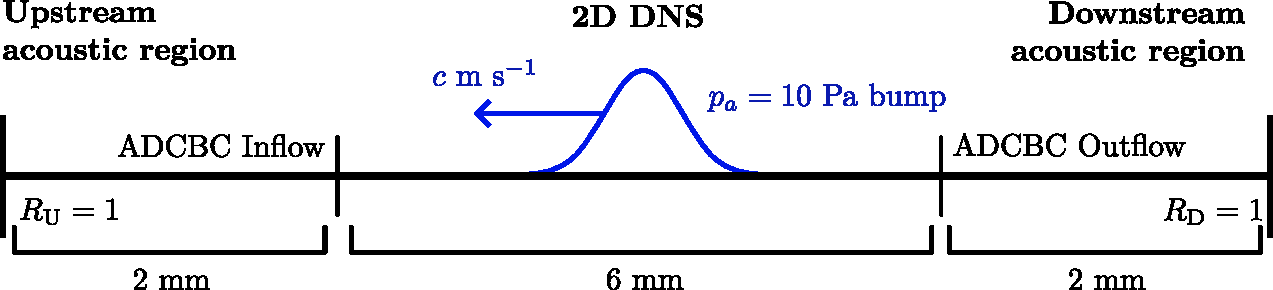
\includegraphics[scale=0.65]{assets/imgs/adcbc_bump_test.pdf}
\caption{The geometry and initialisation for the acoustic bump test case. Not drawn to scale.}
\label{fig:ac-bump-test}
\end{figure}

As our first test case, we model a Gaussian acoustic bump in a two-dimensional tube with two closed ends. The test case is initialised as a small bump in $J_1 \approx p' - ρ c u'$ (where the approximation comes from acoustic linearisation):
\begin{equation}
p_a(t = 0, x) = A \exp\left( - x^2 / d^2 \right)
\quad \text{and} \quad
u_a(t = 0, x) = p_a(t = 0, x) / ρ c
\end{equation}
such that the maximum pressure disturbance is $A = 10$ Pa and diameter $d = 2$ mm. This simple linear approximation also results in a small $J_5$ bump which we ignore. Alternate methods approximating this initial disturbance could also be used, although the provide little relevant improvement. Fluid properties are $u_{\rm{IN}} = 0.2$ m s$^{-1}$, $T_{\rm{IN}} = 298$ K and $p_{\rm{IN}} = 0.1$ MPa comprised of a single species with properties $W = 28$ kg kmol$^{-1}$, $Pr = 0.7$ and $c_p = 1100$ J kg$^{-1}$ K$^{-1}$. The resulting sound speed is $c \approx 348$ m s$^{-1}$. A 6 mm long central DNS region is used as well as up- and downstream acoustic regions modelled using ADCBCs on the inflow and outflow respectively, each modelling 2 mm of truncated tube. These essentially model two one-dimensional acoustic regions to the left and right of the flame. A diagram for this test case is shown in \fig{fig:ac-bump-test}. A sample rate of $δt_{\rm{sample}} \approx 0.25$ {\textmu}s is used for both ADCBCs and we use \nth{0} order interpolation (constant sample values) at the moment, for reasons discussed later. The horizontal top and bottom boundaries used in the DNS region are symmetric mirror boundaries, 1 mm apart. In total, there are 1224 collocation points in this domain processed by a single processor and 11 boundary nodes per boundary. With the linear acoustics equations in the acoustic regions being non-dispersive, we expect the Gaussian to retain its shape after each up- and downstream bounce. The full reacting Navier-Stokes equations are solved in the DNS region as a precursor to the a flame being present in the DNS region. Only in the DNS region should viscous effects alter the wave packet's shape and even in this case, only slightly after many bounces back and forth the 1 cm long domain. The ADCBCs work almost identically when the viscous inert, isothermal equations, which are also implemented into the SUNSET code, are solved. Note that the response to transverse effects are not being tested here because the acoustic is entirely one-dimensional. As mentioned above, we should in fact be modelling the convected wave equation, not the wave equation for quiescent fluids. But, since our Mach number, $\Ma < 10^{-3}$ is so low in this case the convective effects are deemed to be asymptotically unimportant. For thin regions like these, the boundary averaging procedure makes some physical sense as transverse behaviour at the boundaries of longer computational domains would be negligible, as it is here under our artificial test case. As the DNS domain widens, however, it seems reasonable that this averaging would result in more and more inaccuracy and potential instability. Hence, the queues are used for each boundary node should instead be used in this case to model many separate one-dimensional acoustic domains for each node. For all the cases in this report, the boundary averaging procedure is used and we find reassuring results regardless.

\begin{figure}[t]
\centering
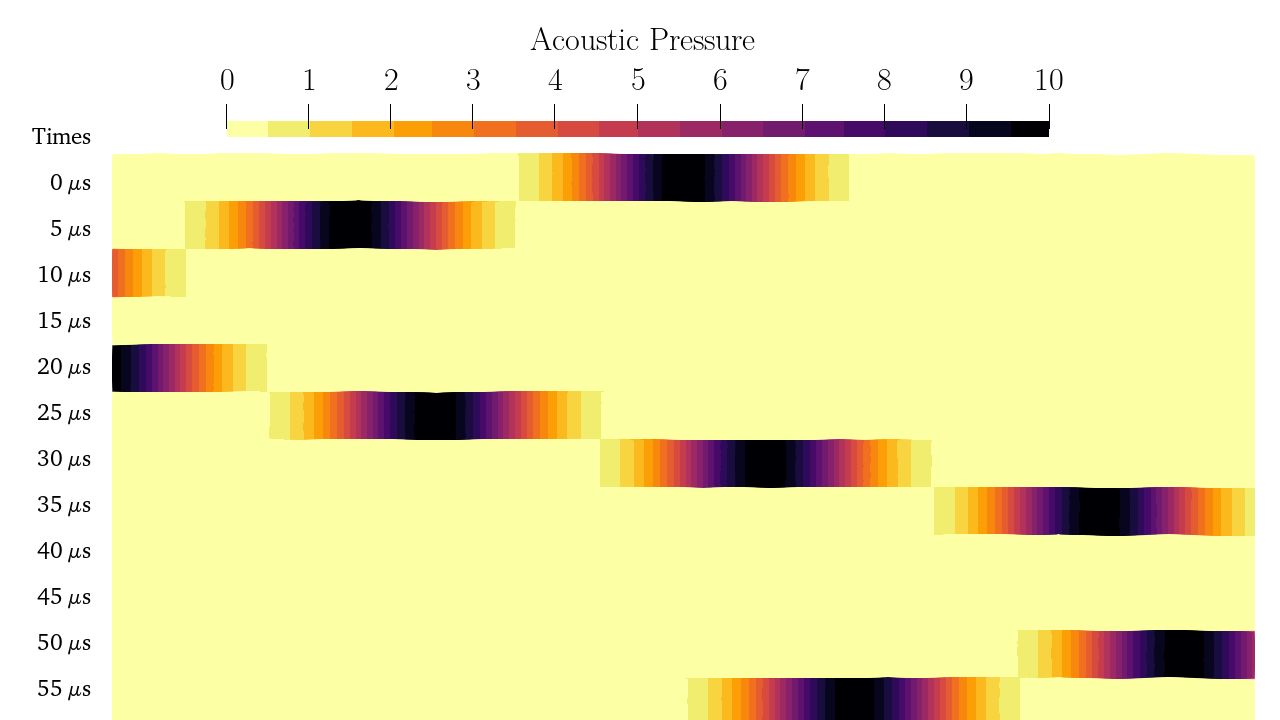
\includegraphics[scale=0.36]{assets/graphs/AC_BUMP_first_bounces_comp.png}
\caption{Acoustic pressure fields in the first 55 {\textmu}s in the DNS region in Pa. Only the top half of each DNS region is shown for comparison.}
\label{fig:ac-bump-dns}
\end{figure}

\begin{figure}[t]
\centering
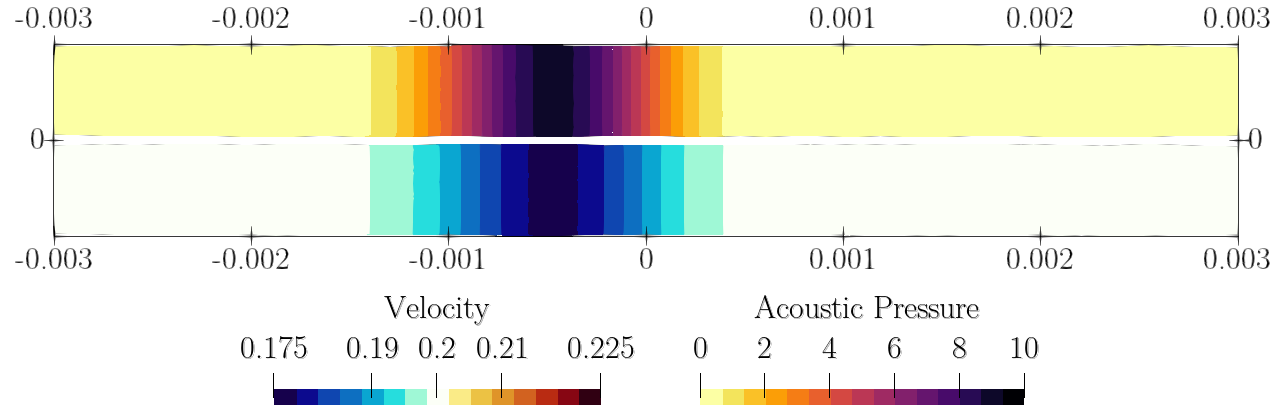
\includegraphics[scale=0.36]{assets/graphs/AC_BUMP_ndt=150e-4_comp.png}
\caption{$p_a$ and $u$ fields after 750 {\textmu}s in Pa and m s$^{-1}$. Here $u_a < 0$ so the acoustic is travelling left.}
\label{fig:ac-bump-dns-late}
\end{figure}

Pressure fields for the first bounces off the up- and downstream acoustic boundary are shown in \fig{fig:ac-bump-dns}. It seems after a single bounce off each end that the ADCBCs are adequately sampling and reintroducing the acoustic bump with negligible changes to its shape. The sample rate means that roughly $(d / c) / δt_{\rm{sample}} \approx 23$ samples are used to sample the first standard deviation of width of the Gaussian. This reconstruction of acoustic shape is impressive given the lack of interpolation (\nth{0} order interpolation means using constant sample values) used. After 750 {\textmu}s, the acoustic should have been sampled by the ADCBCs and reentered the DNS domain 13 times through each boundary. Note that up to this point in the simulation, the boundary conditions have taken up less than one percent of the overall simulation runtime. This is unsurprising given how few boundary nodes there are and since the bulk of the simulation time is spent calculating gradients at the other $\sim$1000 discretisation points. The pressure and velocity fields are shown in the DNS region at this time in \fig{fig:ac-bump-dns-late}. We can see that the size of highest acoustic pressure region has shrunk somewhat so some acoustic losses have been encountered. We note here that a better test of the ADCBCs would be to compare these results against a fully simulated 1 cm long tube with hard inflows and outflows given by specifying $u=0.2$ m s$^{-1}$ at these boundaries to model the closed boundaries. This analysis is not performed in this report. Regardless, it seems as though changes to the acoustic's shape are minimal despite the short acoustic length scale. Thus, from the previous chapter we know that this error should be minimised even farther when a longer tube is simulated. For example, if a 1 m long tube is simulated instead, we expect the same error to occur at roughly $t_C = (1~\text{m} / 1~\text{cm})^2 \cross 750~\text{{\textmu}m} = 7.5$ s in the longer simulation. This should be ample time to simulate a thermoacoustically unstable flame.

\begin{figure}[t]
\centering
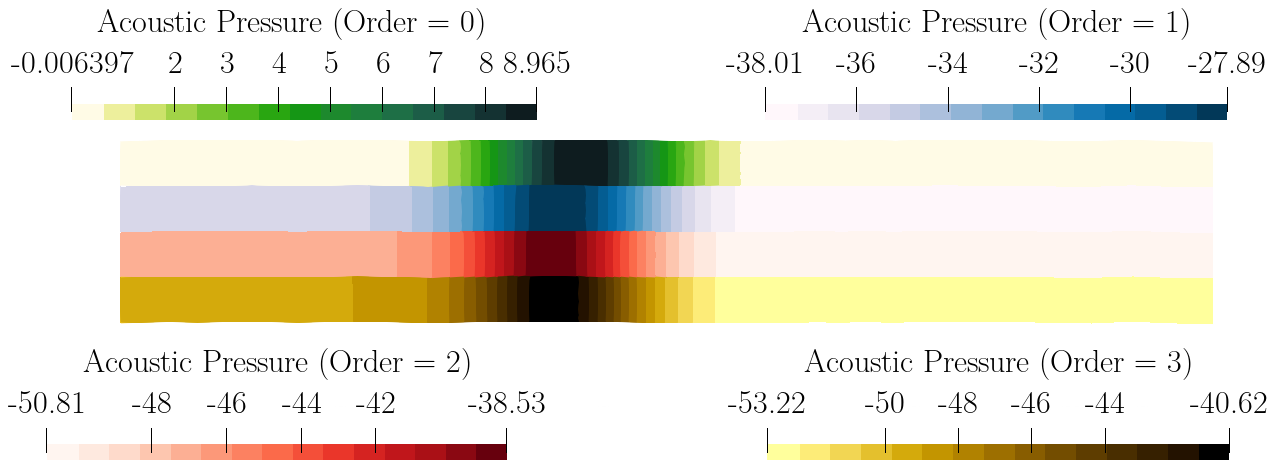
\includegraphics[scale=0.36]{assets/graphs/AC_BUMP_orders.png}
\caption{Acoustic pressures of the acoustic disturbance after 750 {\textmu}s for zero to third order interpolation (top to bottom) in Pa. Only the top half of each DNS region is shown for comparison.}
\label{fig:ac-bump-dns-orders}
\end{figure}

The above results are found provided constant interpolation is used to evaluate $\overline{\cl{L}}(t - τ)$ values. Results of the same Gaussian acoustic bump after 750 {\textmu}s for orders zero to three are shown in \fig{fig:ac-bump-dns-orders}. Bizarrely, when higher orders of interpolation are used the results massively deteriorate and large amounts of error are introduced each every bounce. After the thirteen bounces, we are left with an acoustic bump of roughly the same size $\max(p_a) - \min(p_a) \approx 10$ Pa, but with a drift in pressure much larger than this. Clearly this pressure drift is the result of the pressure difference between the front and back of the bump adding up after repeated bounces, which is most likely caused by the sampling error introduced in the previous chapter since the boundary averaging procedure should be having little to no effect in this quasi-one-dimensional test case. Although, it is unclear why this happens only when non-constant interpolation is used. Assuming it isn't the result of a mistake in the ADCBCs implementation into the SUNSET code, there is potentially some term in the error of the reintegrated acoustic upon reentry which is cancelled out when constant sample values are used, but not for interpolated values. Either way, this needs to be investigated further.

\begin{figure}[t]
\centering
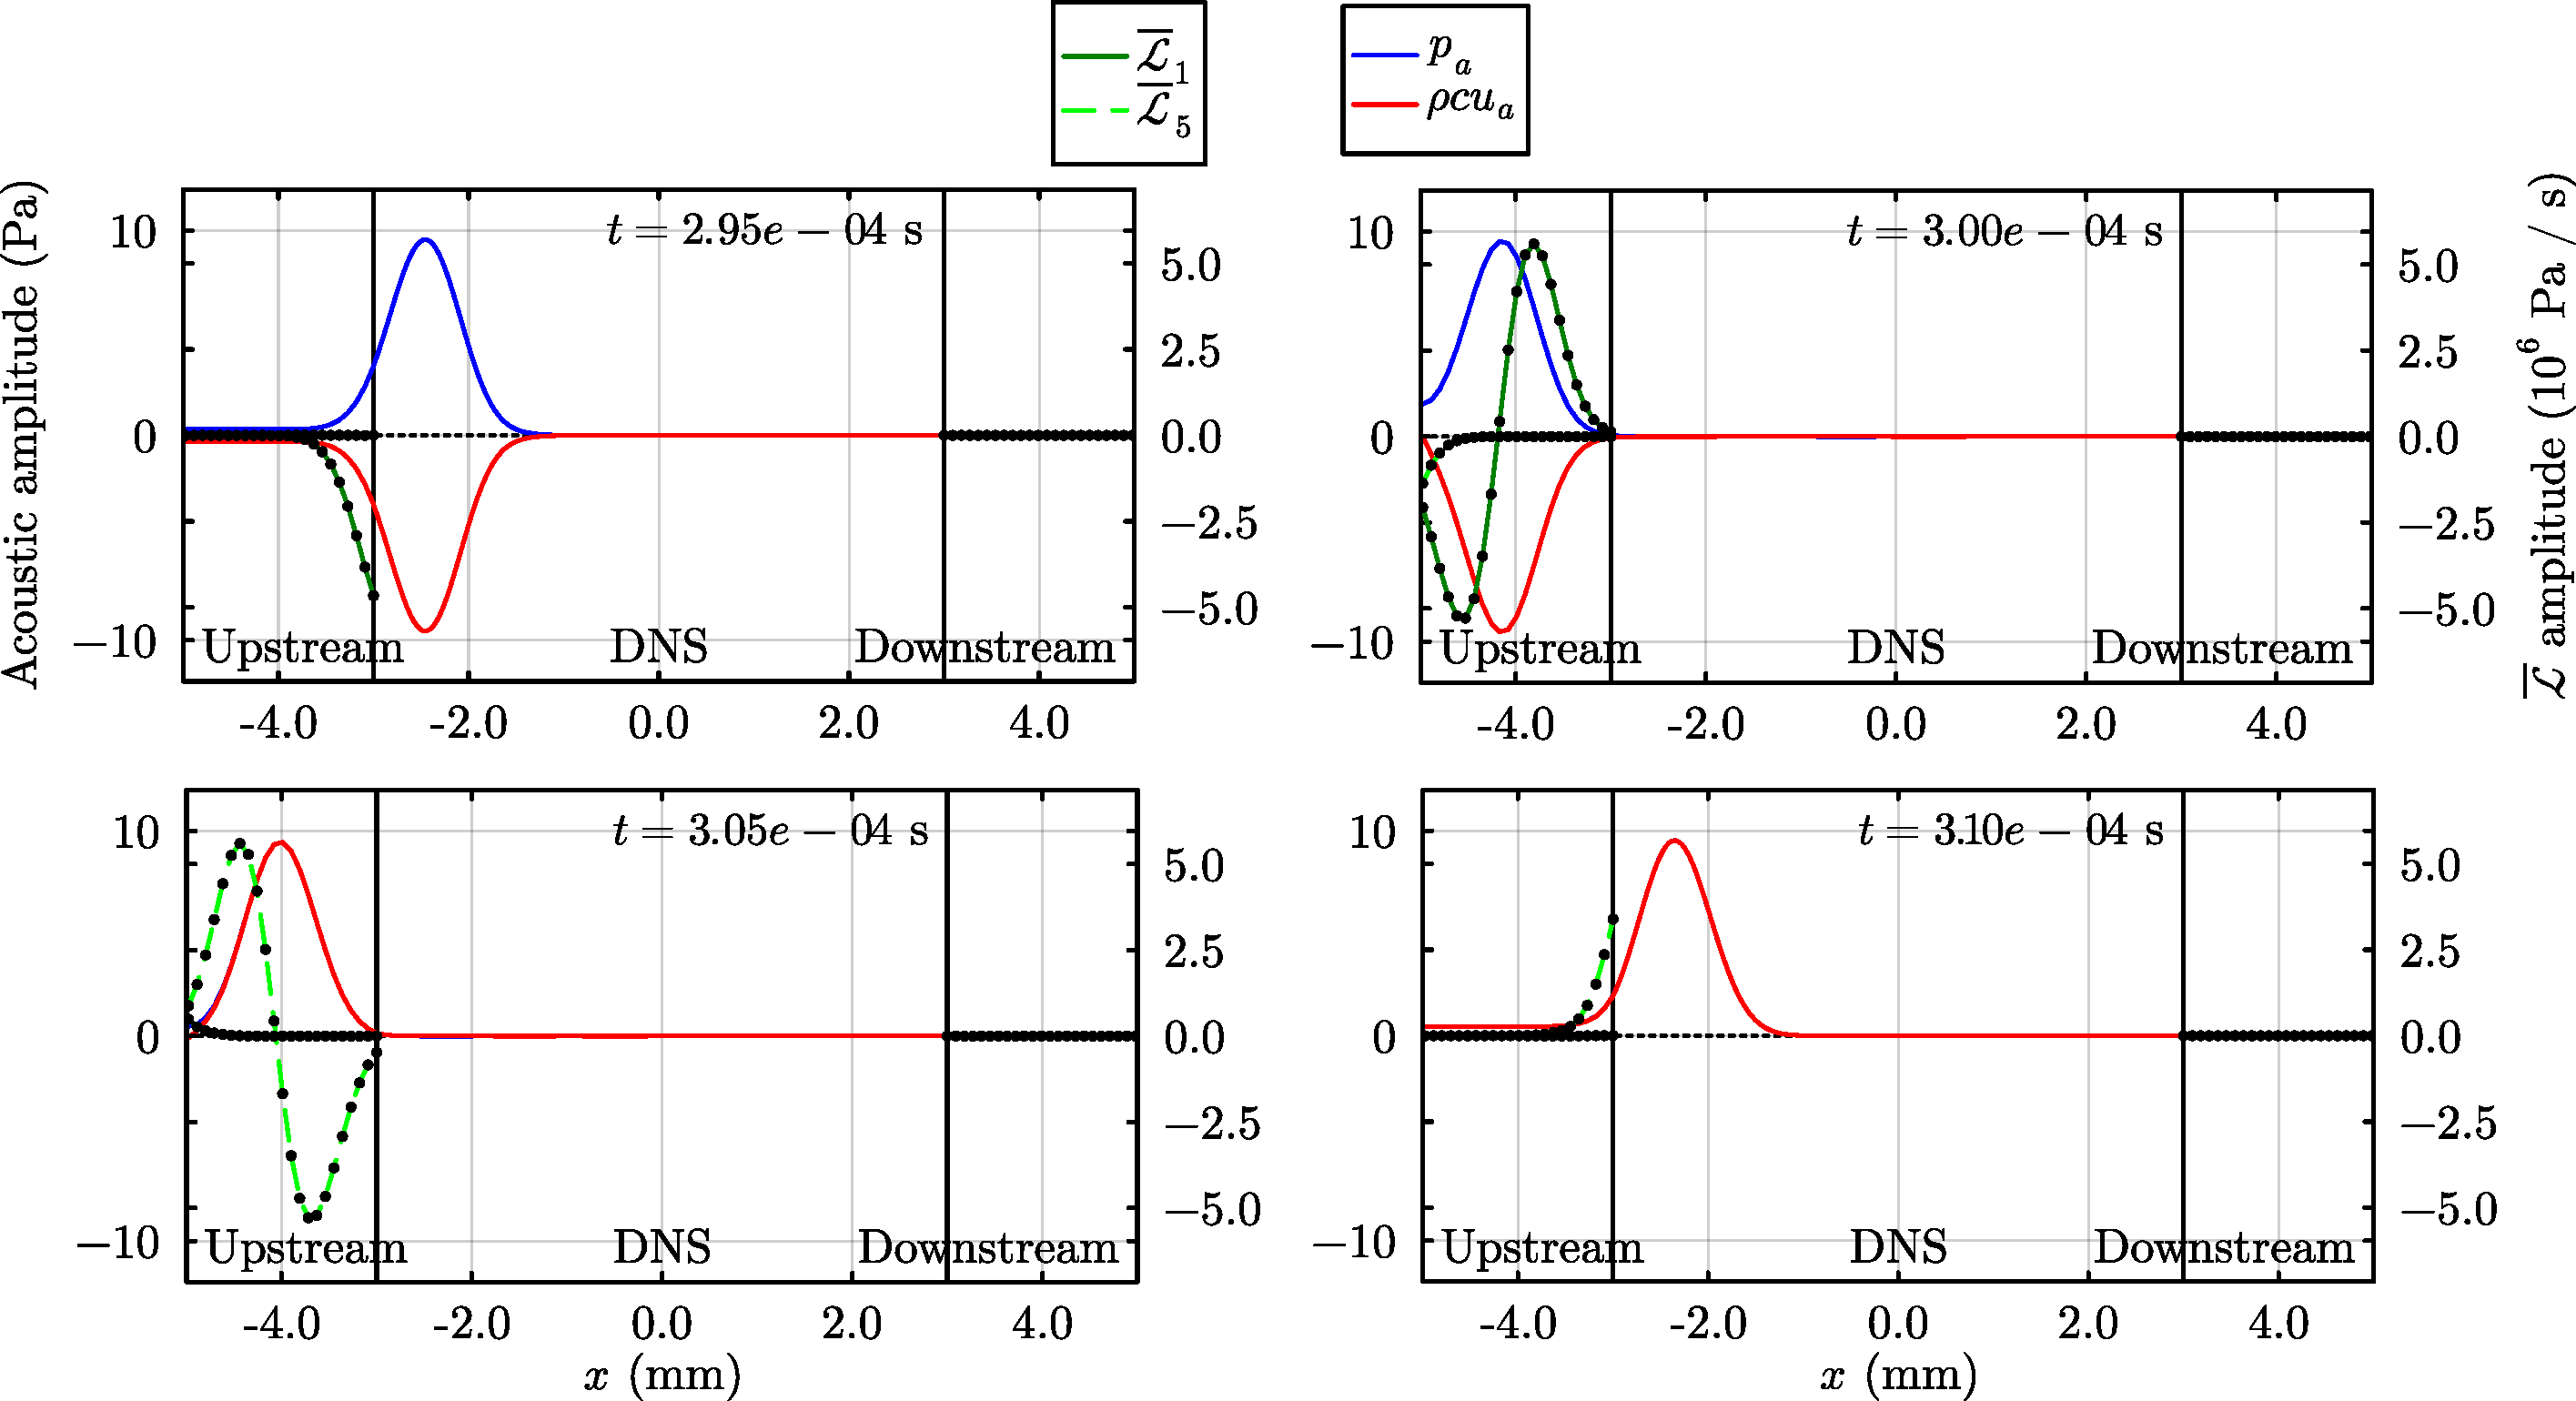
\includegraphics[scale=0.35]{assets/graphs/ac_frames_order=0.pdf}
\caption{Reconstruction of the acoustic fields in the acoustic and DNS regions for the simulation using zeroth order interpolated samples.}
\label{fig:ac-reconstruct_order0}
\end{figure}

\begin{figure}[t]
\centering
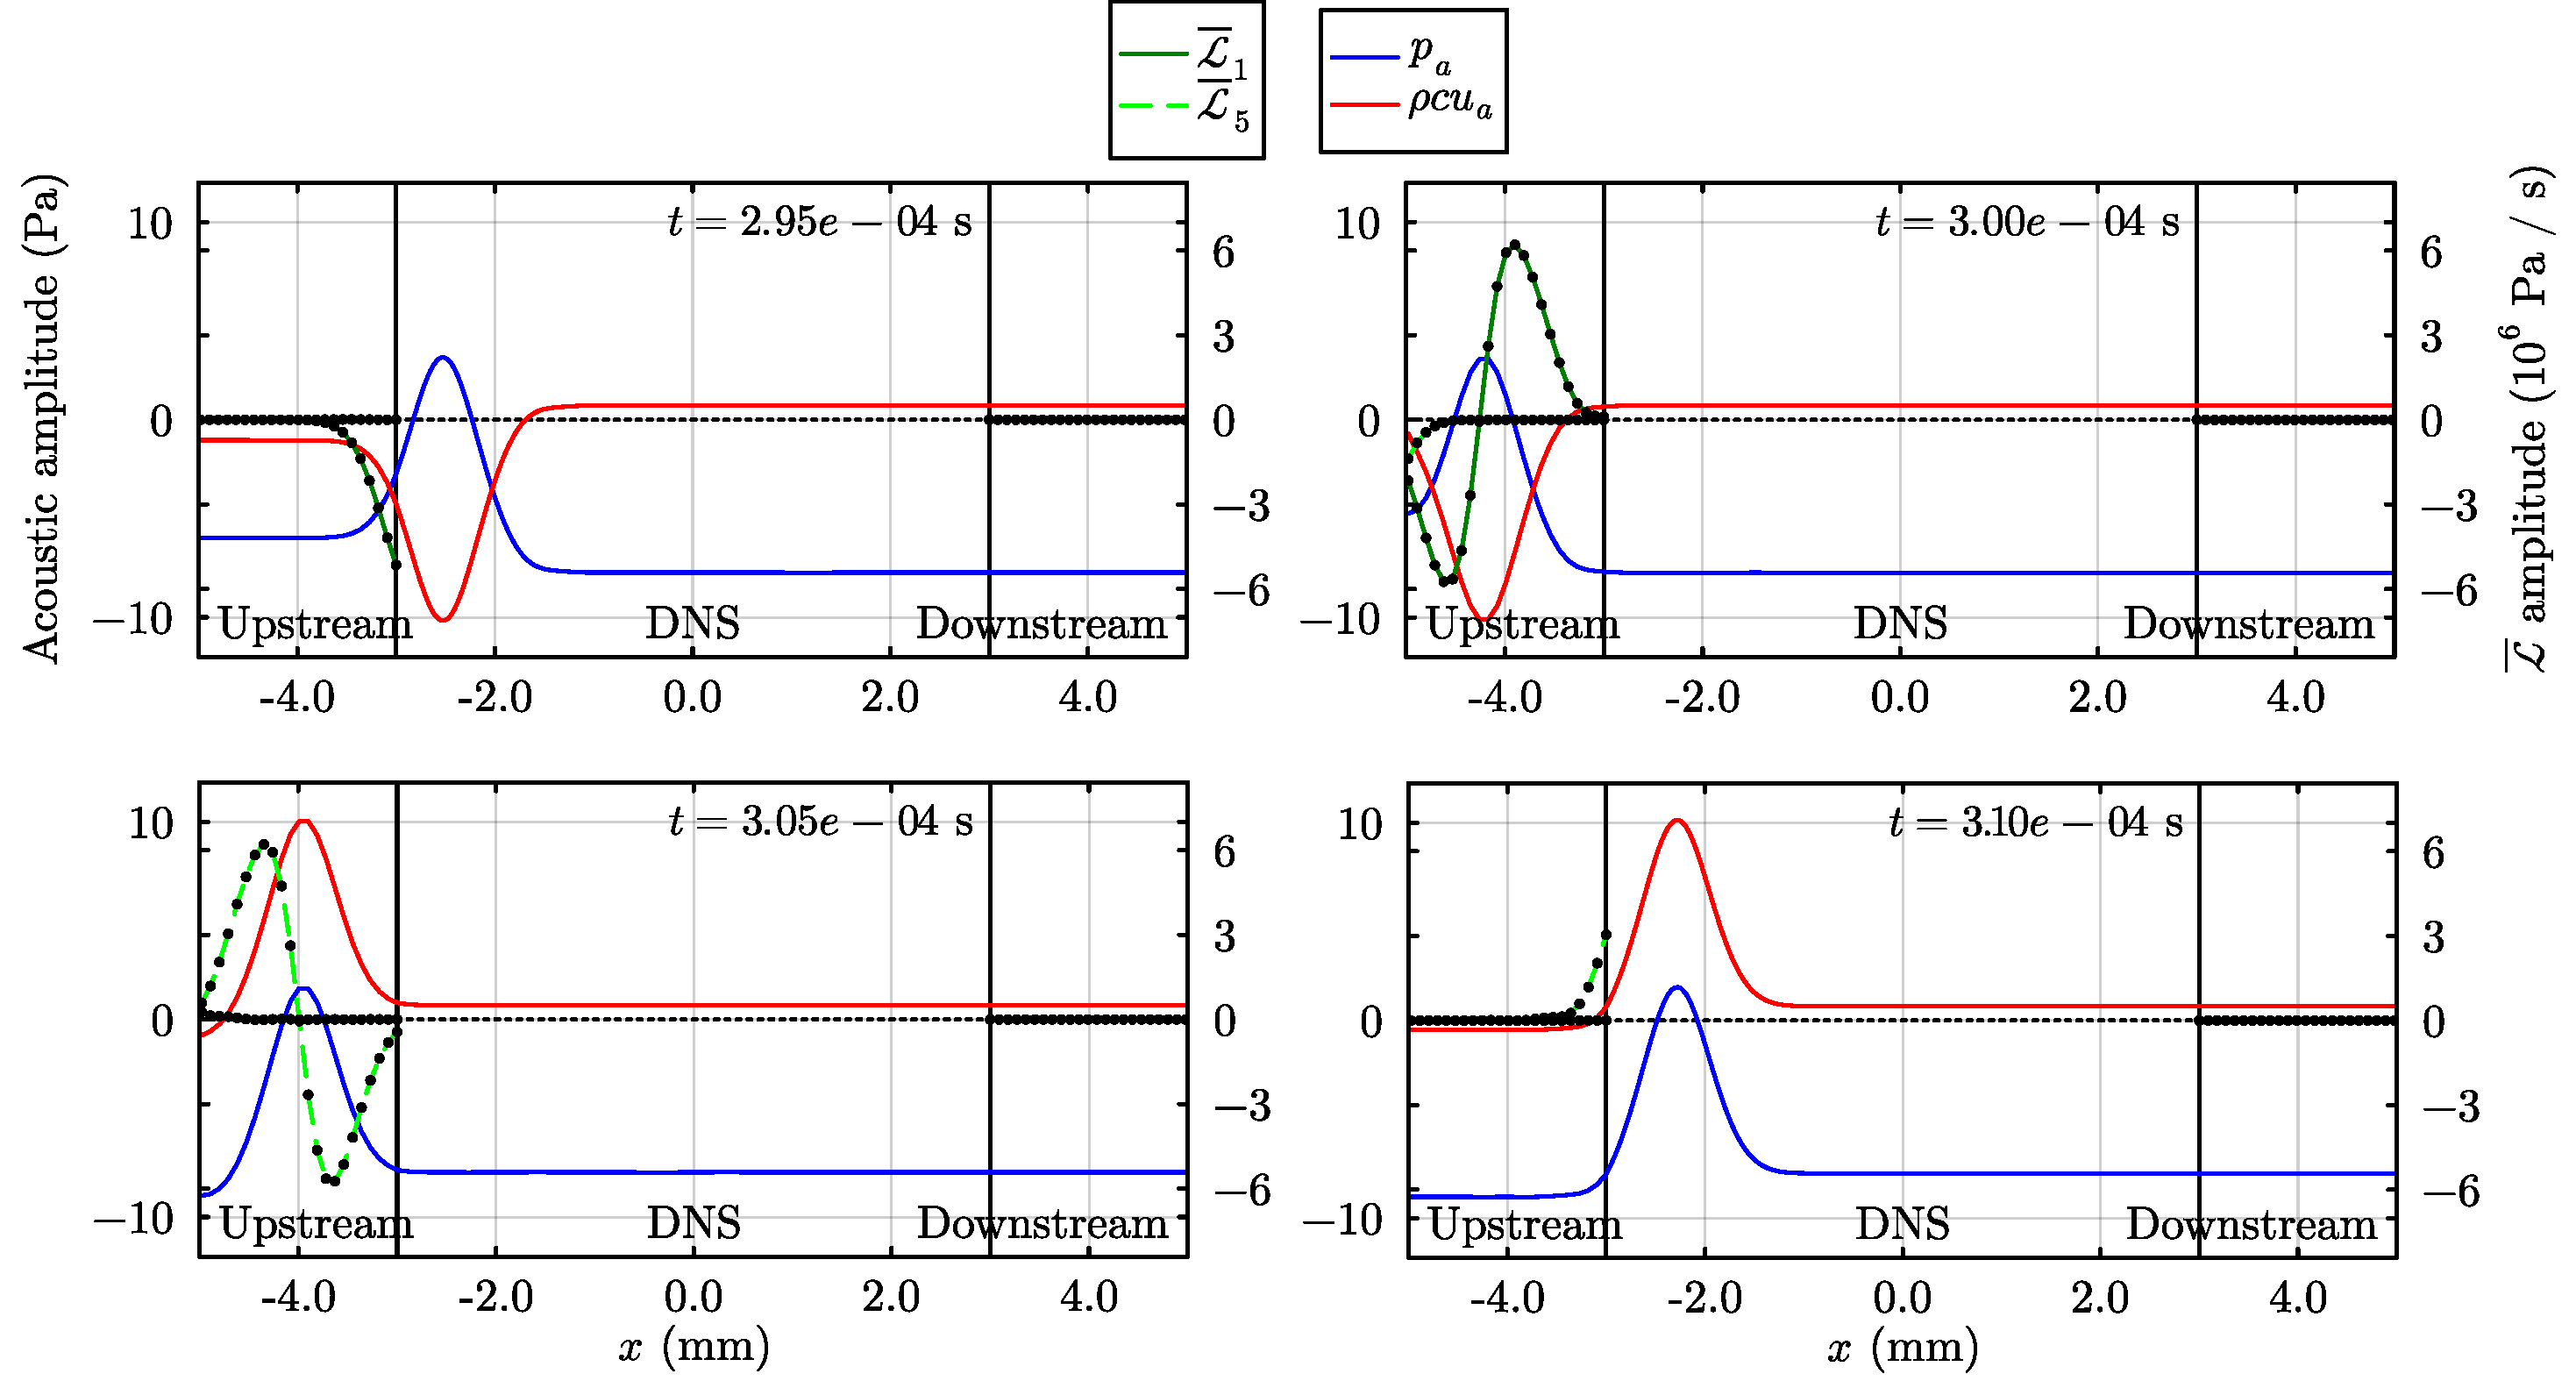
\includegraphics[scale=0.35]{assets/graphs/ac_frames.pdf}
\caption{Reconstruction of the acoustic fields in the acoustic and DNS regions for the simulation using third order interpolated samples.}
\label{fig:ac-reconstruct_order3}
\end{figure}

We can now use the discretised acoustic region field reconstruction from the previous chapter to observe the acoustics in the fictitious region in a way which is not immediately available to us from the interior DNS data. In \fig{fig:ac-reconstruct_order0} are the results for the constant interpolation, where we see although the acoustic field has dissipated by $\sim$1 Pa, the symmetric Gaussian structure is maintained. Instead, in \fig{fig:ac-reconstruct_order3} an asymmetric structure resulting in the pressure drift mentioned above. The values of $\cl{L}$ in both figures showcase these values moving with $p_a$ and $u_a$ in the upstream acoustic domain, which is roughly $\propto ζ \exp(-ζ^2)$ for some variable $ζ(t, x)$. Notice that because $R_{\rm{U}} = 1$ in both cases we get that $\cl{L}_{5, \rm{U}}(t, x_{\rm{IN}} - l_{\rm{U}}) = \cl{L}_{1, \rm{U}}(t, x_{\rm{IN}} - l_{\rm{U}})$. This should always result in the Dirichlet condition $u_a(t, x_{\rm{IN}} - l_{\rm{U}}) = 0$ and Von Neumann condition $\partial p_a / \partial x(t, x_{\rm{IN}} - l_{\rm{U}}) = 0$, althoug we notice that this is not true for the third order simulation. In the case where an open acoustic boundary $R_{\rm{U}} = -1$ is used instead, we have $\cl{L}_{5, \rm{U}}(t, x_{\rm{IN}} - l_{\rm{U}}) = -\cl{L}_{1, \rm{U}}(t, x_{\rm{IN}} - l_{\rm{U}})$ so the boundary conditions on $p_a$ and $u_a$ swap. Both these cases match the desired acoustic properties for open and closed tubes under typical acoustic modelling.




\section{Acoustic Standing Wave}

\begin{figure}[t]
\centering
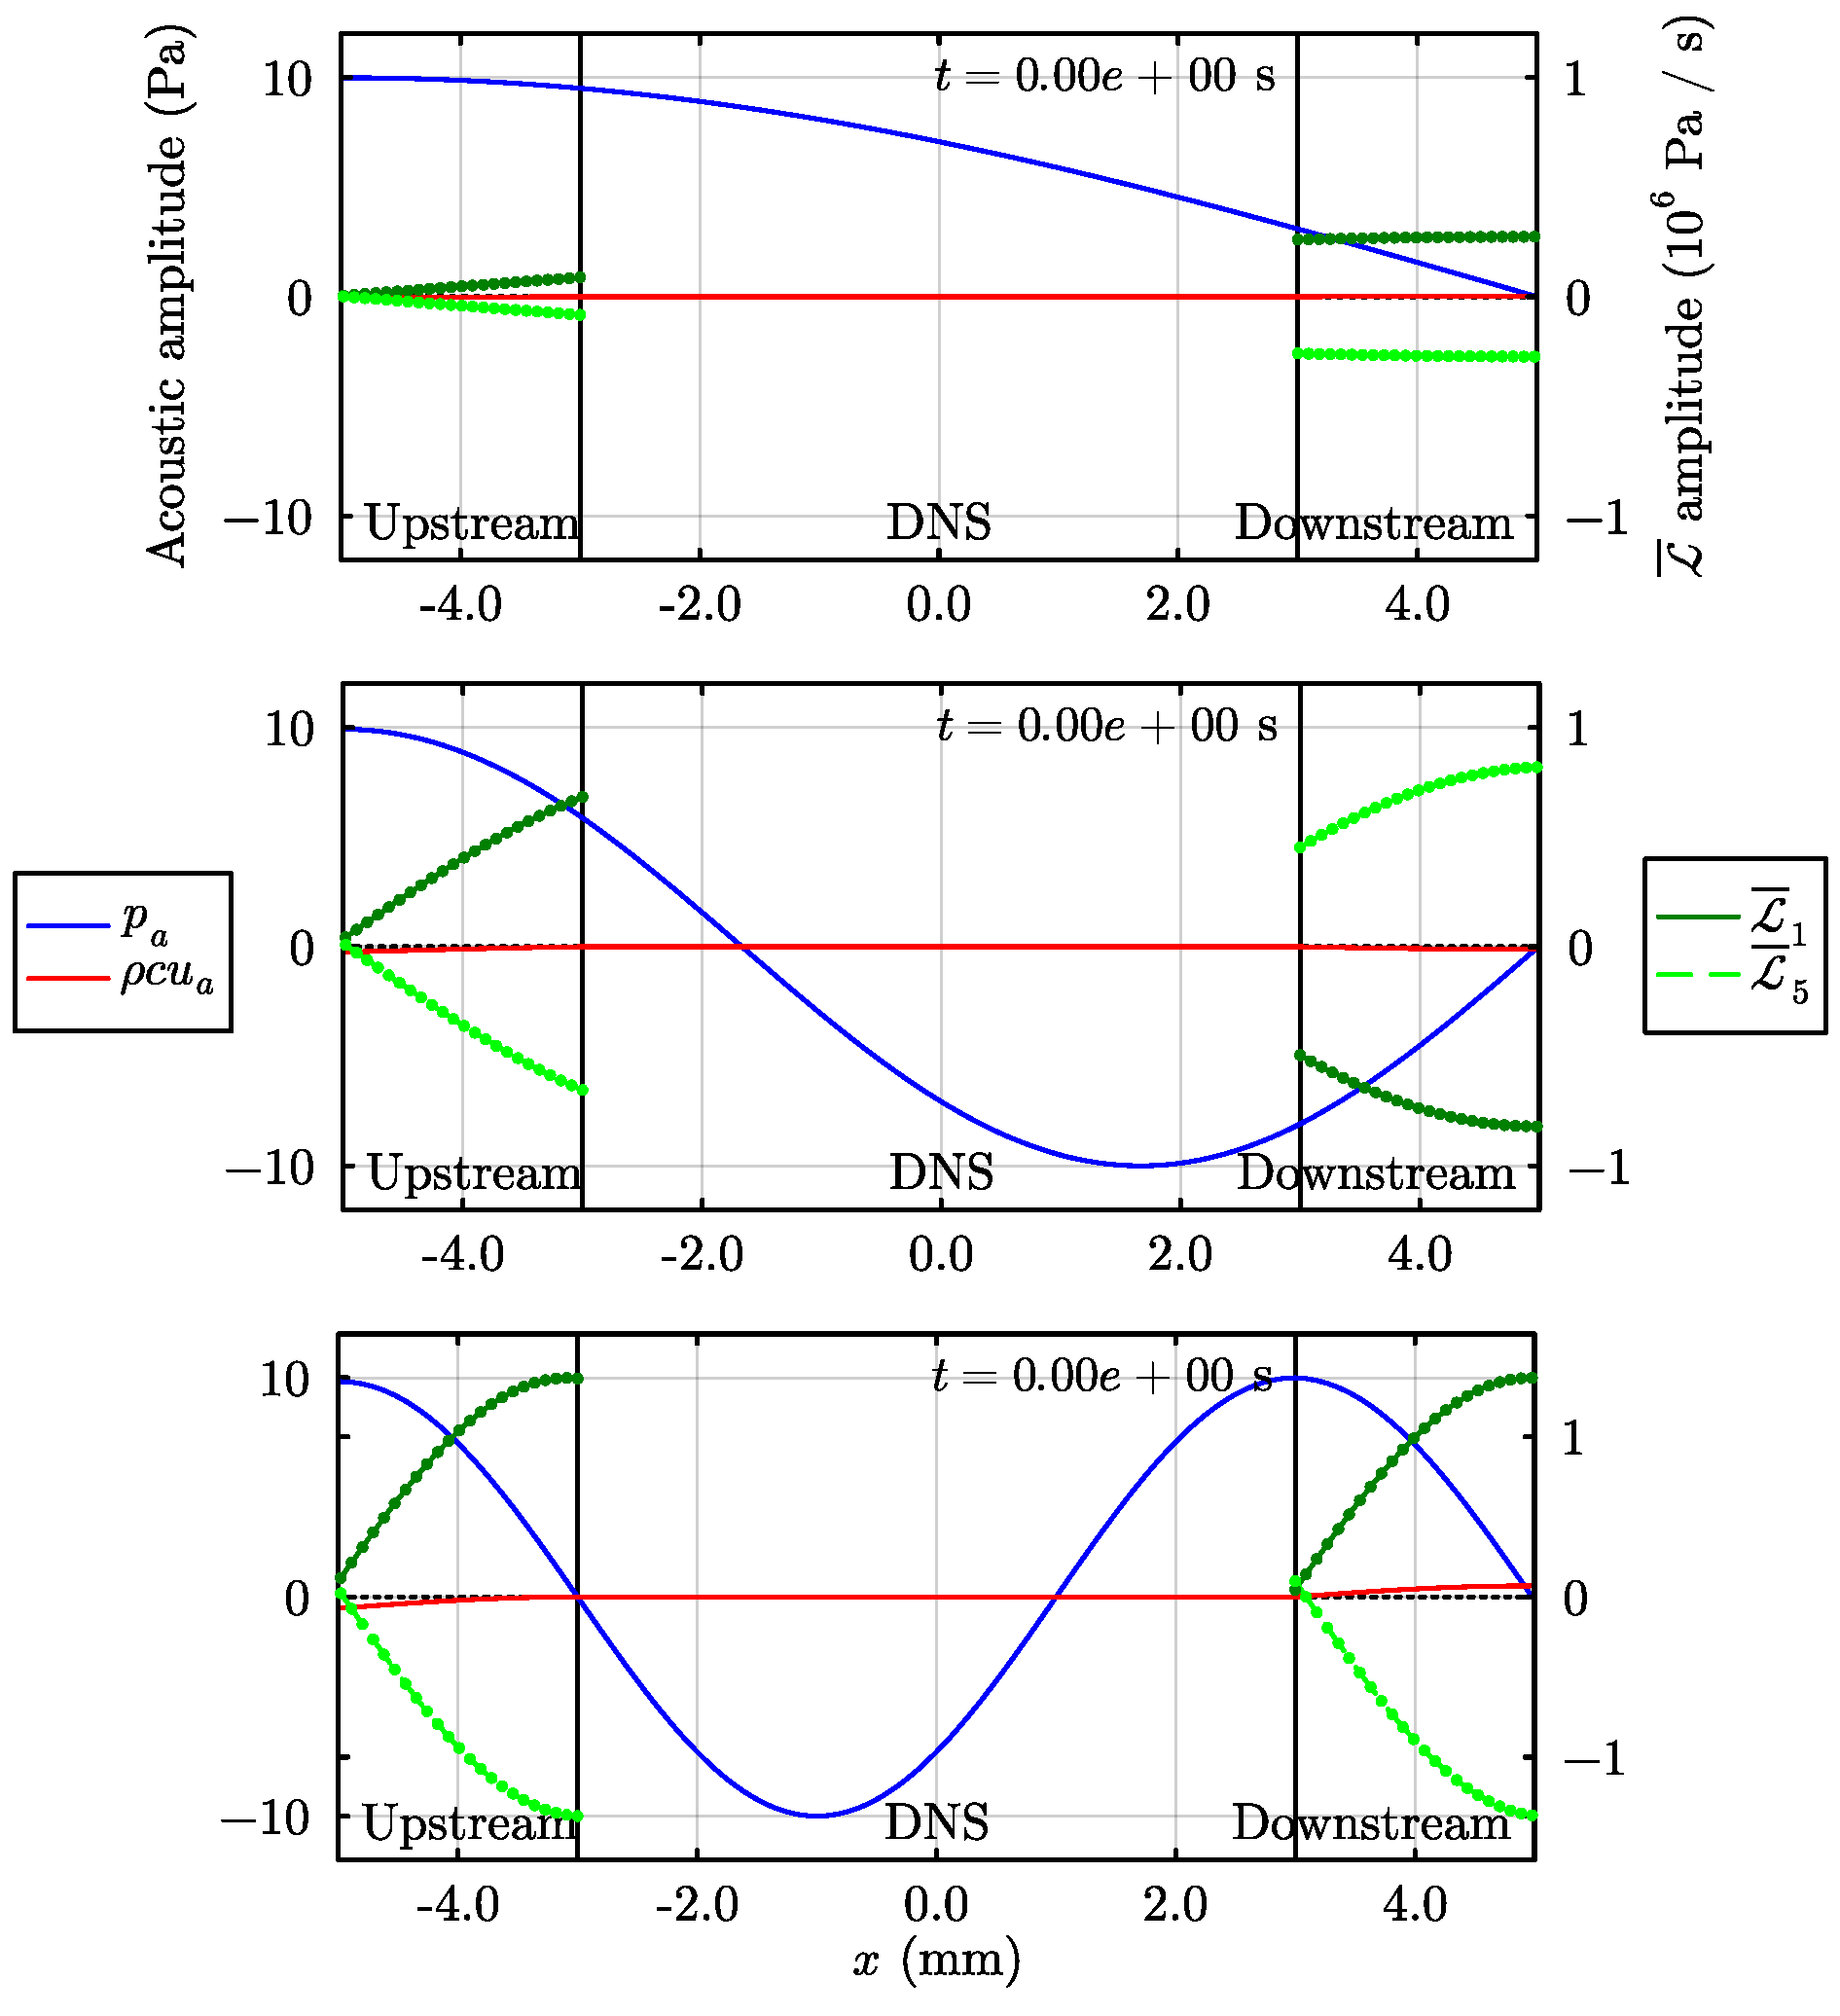
\includegraphics[scale=0.35]{assets/graphs/ac-plot-wave-modes.pdf}
\caption{Reconstruction of the initial acoustic fields for $N_κ = 1, 2, 3$.}
\label{fig:ac-wave-modes}
\end{figure}

\begin{figure}[t]
\centering
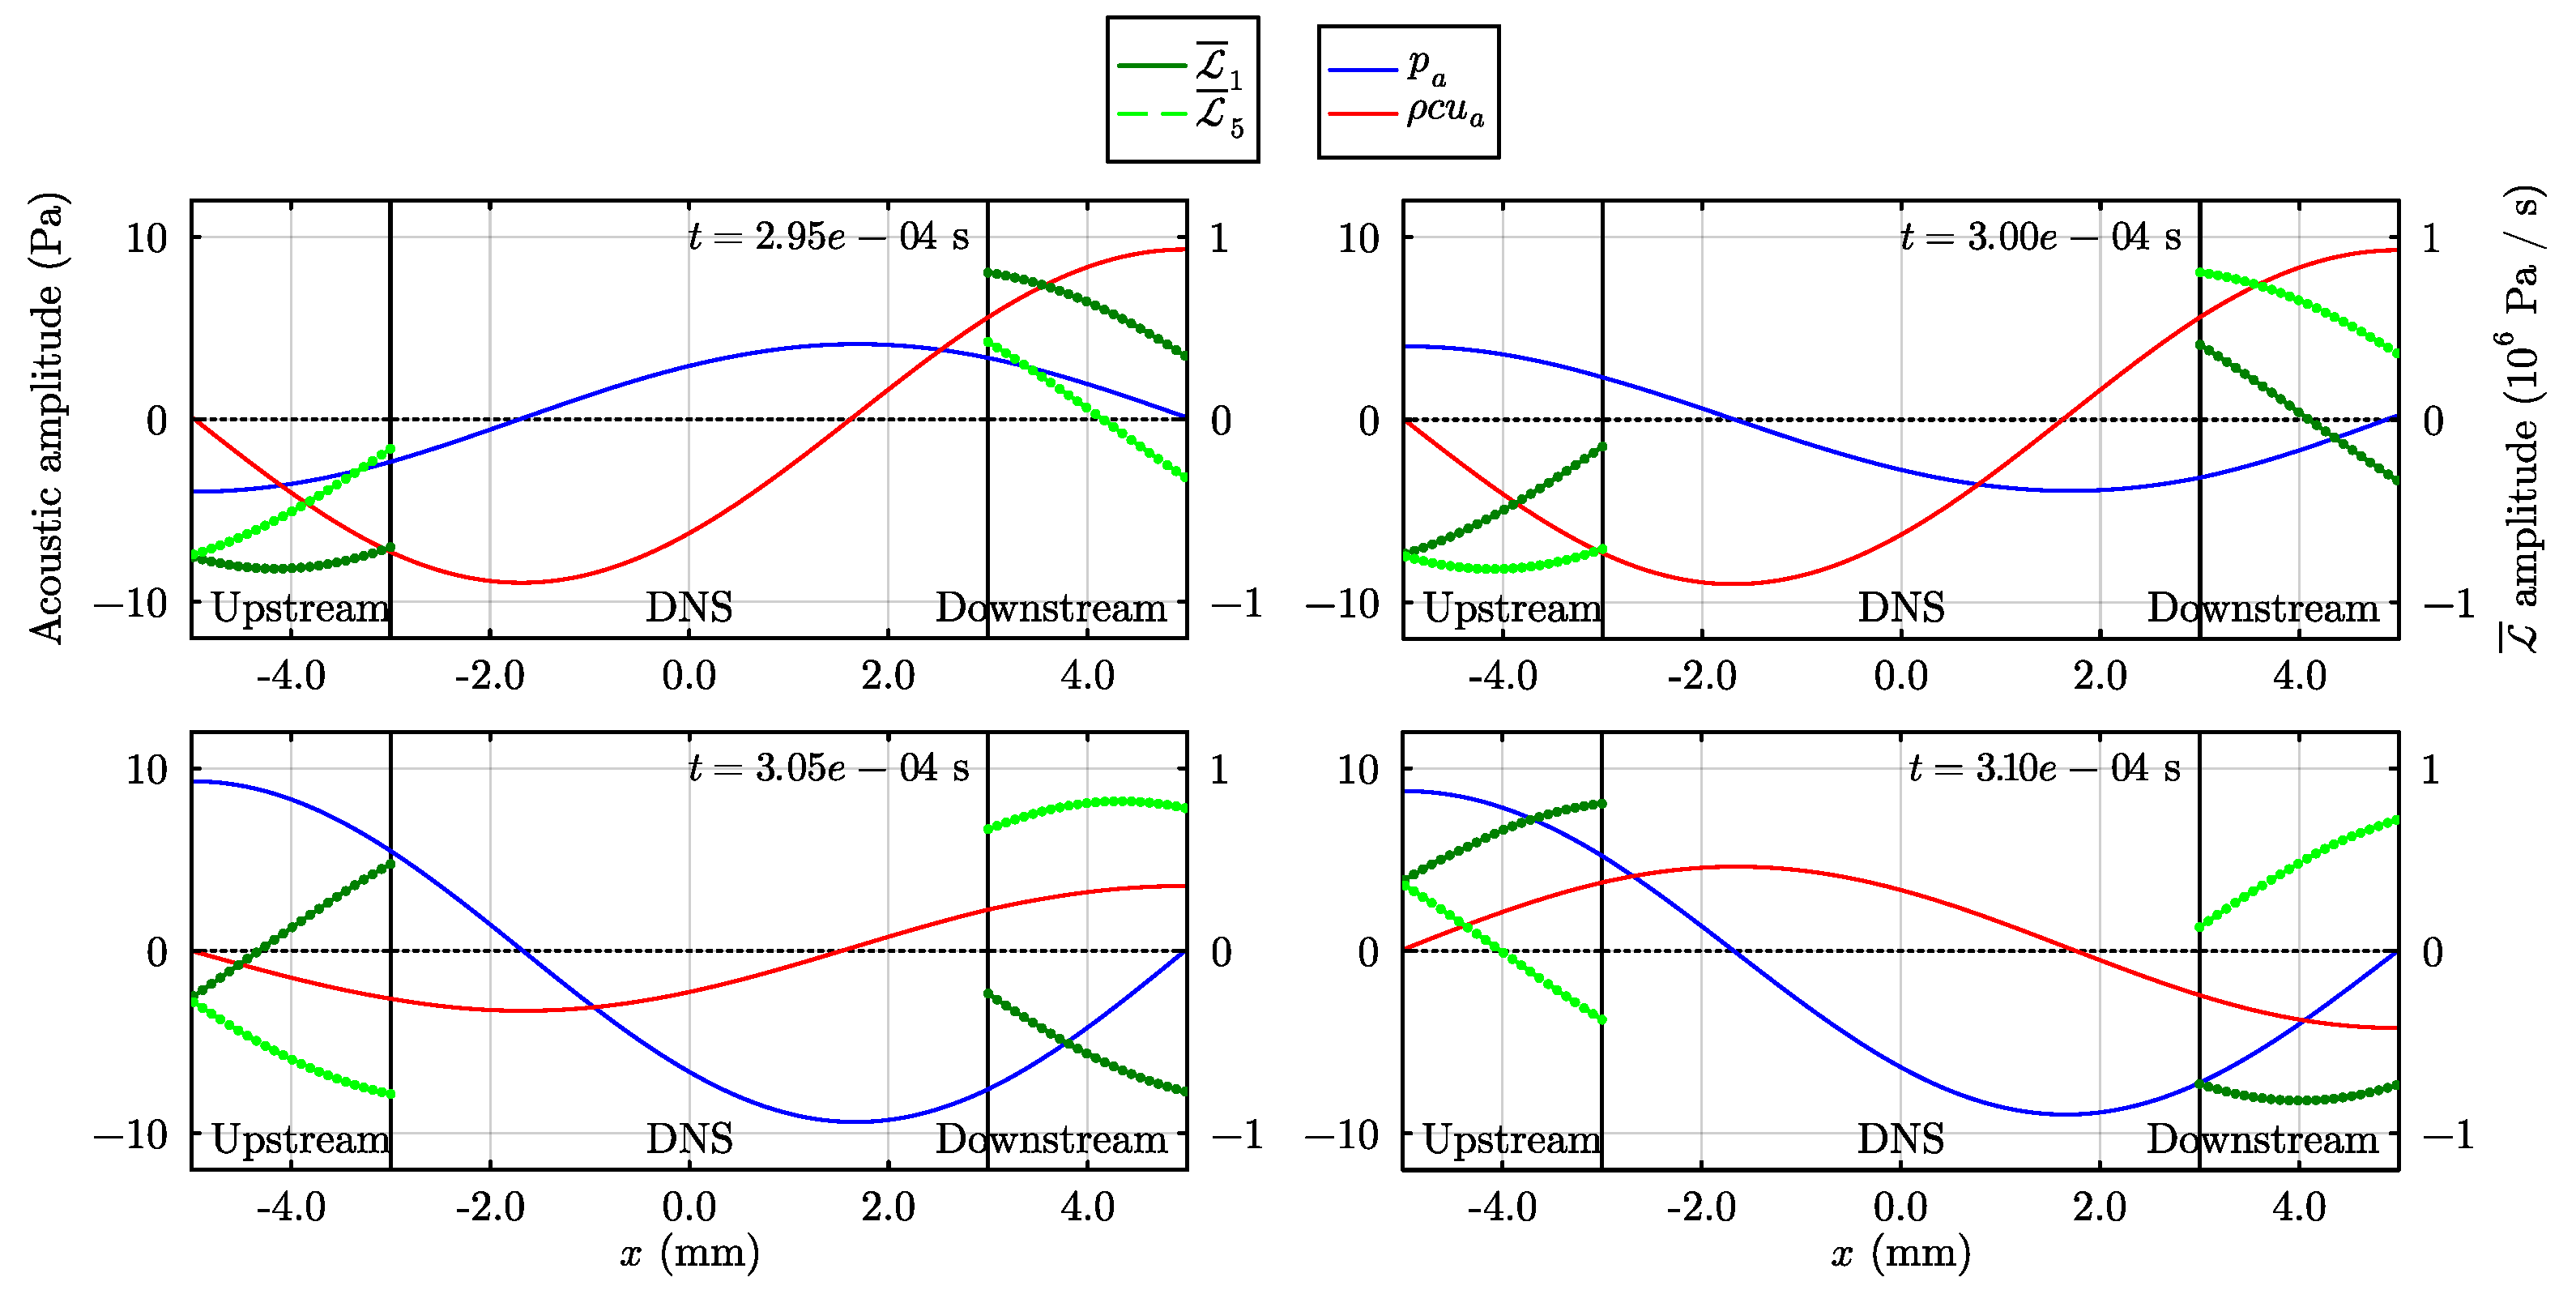
\includegraphics[scale=0.33]{assets/graphs/ac-plot-3-4_long.pdf}
\caption{Reconstruction of acoustic fields for $N_κ = 2$.}
\label{fig:ac-wave-later}
\end{figure}

We now initialise an acoustic standing wave in the same computational domain as the previous test case, using the same fluid properties and ADCBC parameters, except for the change that we instead model an open upstream acoustic boundary, so $R_{\rm{D}} = -1$ instead and we use constant interpolation. The desired initial acoustic pressure is:
\begin{equation}
p_A(t = 0, x) = A \cos\left( 2 π \, \frac{x - x_{\rm{IN}} - l_{\rm{U}}}{l_{\rm{tube}}}  \, \frac{2N_κ - 1}{4}\right),
\end{equation}
where $A = 10$ Pa is the acoustic amplitude as before and $l_{\rm{tube}} \equiv l_{\rm{U}} + (x_{\rm{OUT}} - x_{\rm{IN}}) + l_{\rm{D}}$ is the full tube length with $l_{\rm{U}} = l_{\rm{D}} = 2$ mm and $(x_{\rm{OUT}} - x_{\rm{IN}}) = 6$ mm. $N_k$ determines the wavenumber of the standing wave: if $N_κ = 1$ we have the $1 / 4$ mode, if $N_κ = 2$ we have the $3 / 4$ mode etc.. The corresponding wavenumber is:
\begin{equation}
κ = \frac{2N_κ - 1}{4 l_{\rm{tube}}}
\end{equation}
In the DNS region, the wave can be initialised by directly calculating $p_a(0, x)$ values. In the upstream and downstream region, however, we must instead calculate $\cl{L}_{1/5}(t = 0, x)$ using the formulae in \equ{eqn:λ_l_L}, discretise them and enter the resulting finite values into the initial queues $(\bb{T} \cross \bb{L})(t = 0)$ for the ADCBC inflow and outflow. \fig{fig:ac-wave-modes} shows the acoustic initial conditions in the full tube for the first three standing wave modes. In each of the three graphs, the wave continues smoothly into the acoustic domain owing the acoustic reconstruction introduced in the previous chapter. \fig{fig:ac-wave-later} shows the simulation after a few acoustic periods for the $N_κ = 2$ case. Clearly $u_a(t, x_{\rm{IN}} - l_{\rm{U}}) = 0$ and $p_a(t, x_{\rm{OUT}} + l_{\rm{D}}) = 0$ as desired. In this case you can see the reconstructed $\cl{L}_{1/5}$ fields travelling left and right respectively. Note that in the $N_κ = 2$ and 3 modes you can see a slight error with some $u_a(t = 0, x) \ne$ values in the up and downstream domain due to inaccuracies with the post-processing code.

\begin{figure}[t]
\centering
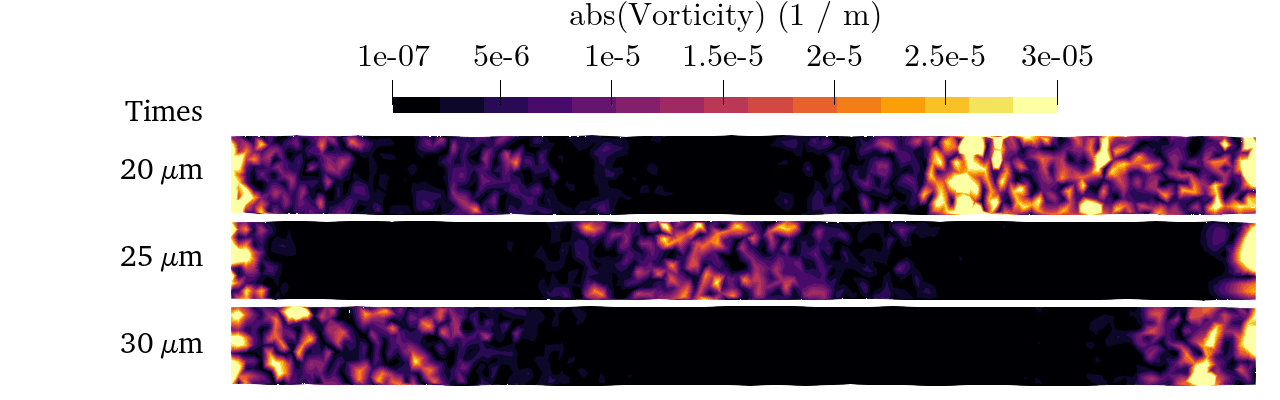
\includegraphics[scale=0.36]{assets/graphs/AC_WAVE_QWAVE.png}
\caption{Spurious vorticity wave travelling through the DNS domain at the acoustic speed for the $N_κ = 2$ wave.}
\label{fig:vort-wave}
\end{figure}

Focusing instead on the DNS region, looking only at vorticity disturbances -- given that the background vorticity should be $\vb{ω} \equiv \vb{\nabla}\cross\vb{u} \equiv 0$ for the one-dimensional flow -- we can see in \fig{fig:vort-wave} a vorticity perturbation travelling at the acoustic speed, right to left. This can also be seen in disturbances to $v$. Not depicted in the figure is this wave and another bouncing back and forth through the DNS domain, as if it is being transmitted through the full acoustic domain. This is likely the result of the $\cl{O}(h^k)$
The simplest explanation for this `error' wave is 
Note the larger values of $\abs{\vb{ω}}$ at the characteristic boundaries due to variations of $u$ and $\cl{L}_{1/5, \rm{nonreflect}}$ along the boundary.

% Sampling error
% - We can also see the sampling instability in the standing wave results as a q-wave \cite{poinsot2001TheoreticalNumericalCombustion} which is largest at maximum values of L???
% - Show image/s. Easiest to see when instability is not present
% - We can find similar results for standing waves as a bump in terms of interpolation order?
% - Once again, for tubes which are long enough this should not be a concern due to the quadratic growth of period with length. This is consistent with our results in the next section



% We use SI units (1 / m)
\begin{figure}[t]
\centering
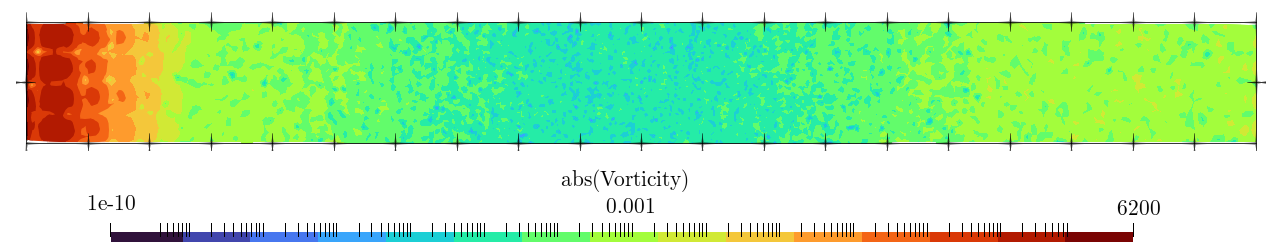
\includegraphics[scale=0.36]{assets/graphs/u-inflow-instab.png}
\caption{INFLOW INSTAB}
\label{fig:inflow-instab}
\end{figure}



% Instability issue!
% - We observed that under certain boundary discretisations, a wringing instability of u develops at the inflow after many acoustic periods. This grows exponentially, suggesting the instability behaves linearly, until the vorticity produced within the DNS region destroys the solution
% - Show image!!
% - This instability can be reduced by increasing the coefficient of the hyperviscosity filter at the inflow boundary nodes. Specifically, by increasing the hyperviscosity tangential to the inflow, the wringing mode is dampened to the point that it cannot grow
% - for us, we..
% - This instability may or may not show up when multiple queues are used for each inflow/outflow, so this needs to be investigated. It appears to be largely a result of the boundary averaging procedure.




% Moving domain results
% - shows validation that the delay time can indeed change
% - time scale for delay change is much longer due to the low Mach number
% - Show two images at separate times where the domain has moved but the acoustic remains well-resolved




\section{Thermoacoustically Unstable Flame}

\begin{figure}[t]
\centering
    \begin{subfigure}{0.99\textwidth}
    \centering
    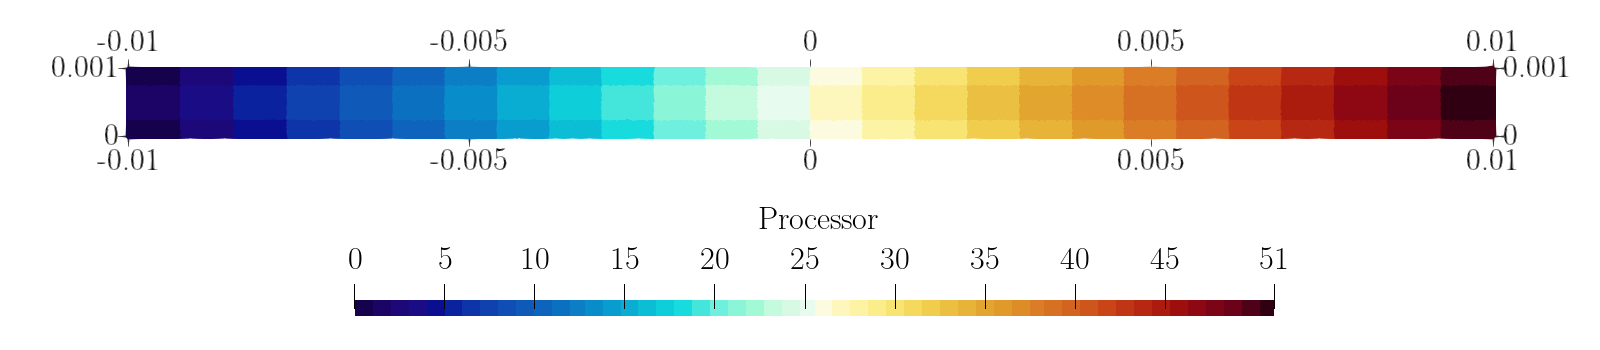
\includegraphics[scale=0.25]{assets/graphs/flame-sim-discretisation.png}
    \caption{}
    \label{fig:disc1}
    \end{subfigure}

\vspace*{0.5em}

    \begin{subfigure}{0.99\textwidth}
    \centering
    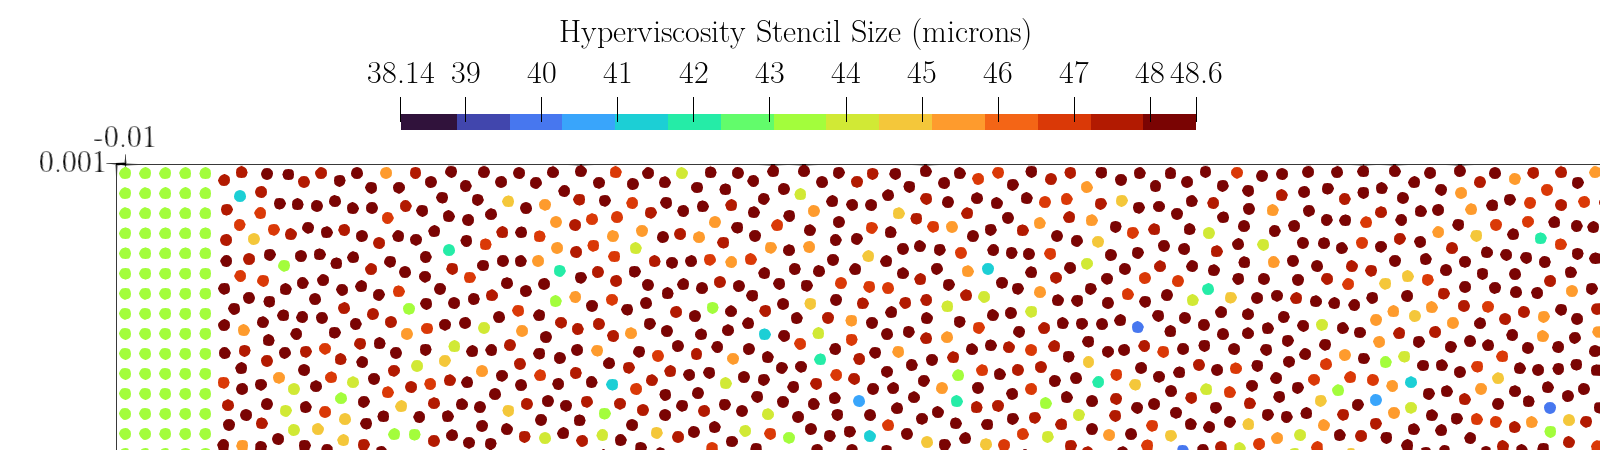
\includegraphics[scale=0.25]{assets/graphs/flame-sim-discretisation_zoom.png}
    \caption{}
    \label{fig:disc2}
    \end{subfigure}
\caption{DNS COMPUTATIONAL DOMAIN}
\label{fig:disc}
\end{figure}

% We now study a thermoacoustically unstable flame in a reflected DNS domain shown in fig ..
% Flame properties are: single step irreversible reaction with fluid properties constant in reactants and products, q = 6, Ze = 5, S_L = u_in = 0.2 m / s, Le = 1, with derived laminar flame thickness l_L = 0.216 mm
% Even though LABFM enables variable resolutions, we use constant discretisation length scale for these simulations as we don't know where the flame will end up a priori. A discretisation length scale of $s = 18$ μm is used and w = 2mm.
% Show the discretisation used zoomed in and out!
% It may seem like a large jump to go from inert, essentially isothermal acoustics to fully reacting flame-acoustic interactions, but the sunset code is designed with flame simulations in mind, so the simulations are 'easy' to perform having already implemented ADCBC.
% (Maybe there are better intermediate test cases? D-TDIBC don't seem to need them)



\subsection{Acoustic Eigenmodes}

% Prediction from Eigenmodes
% - First we predict what results we get in a one-dimensional closed-open tube of the same length under the linear acoustic approximation, modelling the flame as a discontinuity which does not interact with the acoustics.
% First take the non-dimensionalised equations for compressible, inviscid fully non-linear flow:
% ... (continue on with maths)

\begin{figure}[t]
\centering
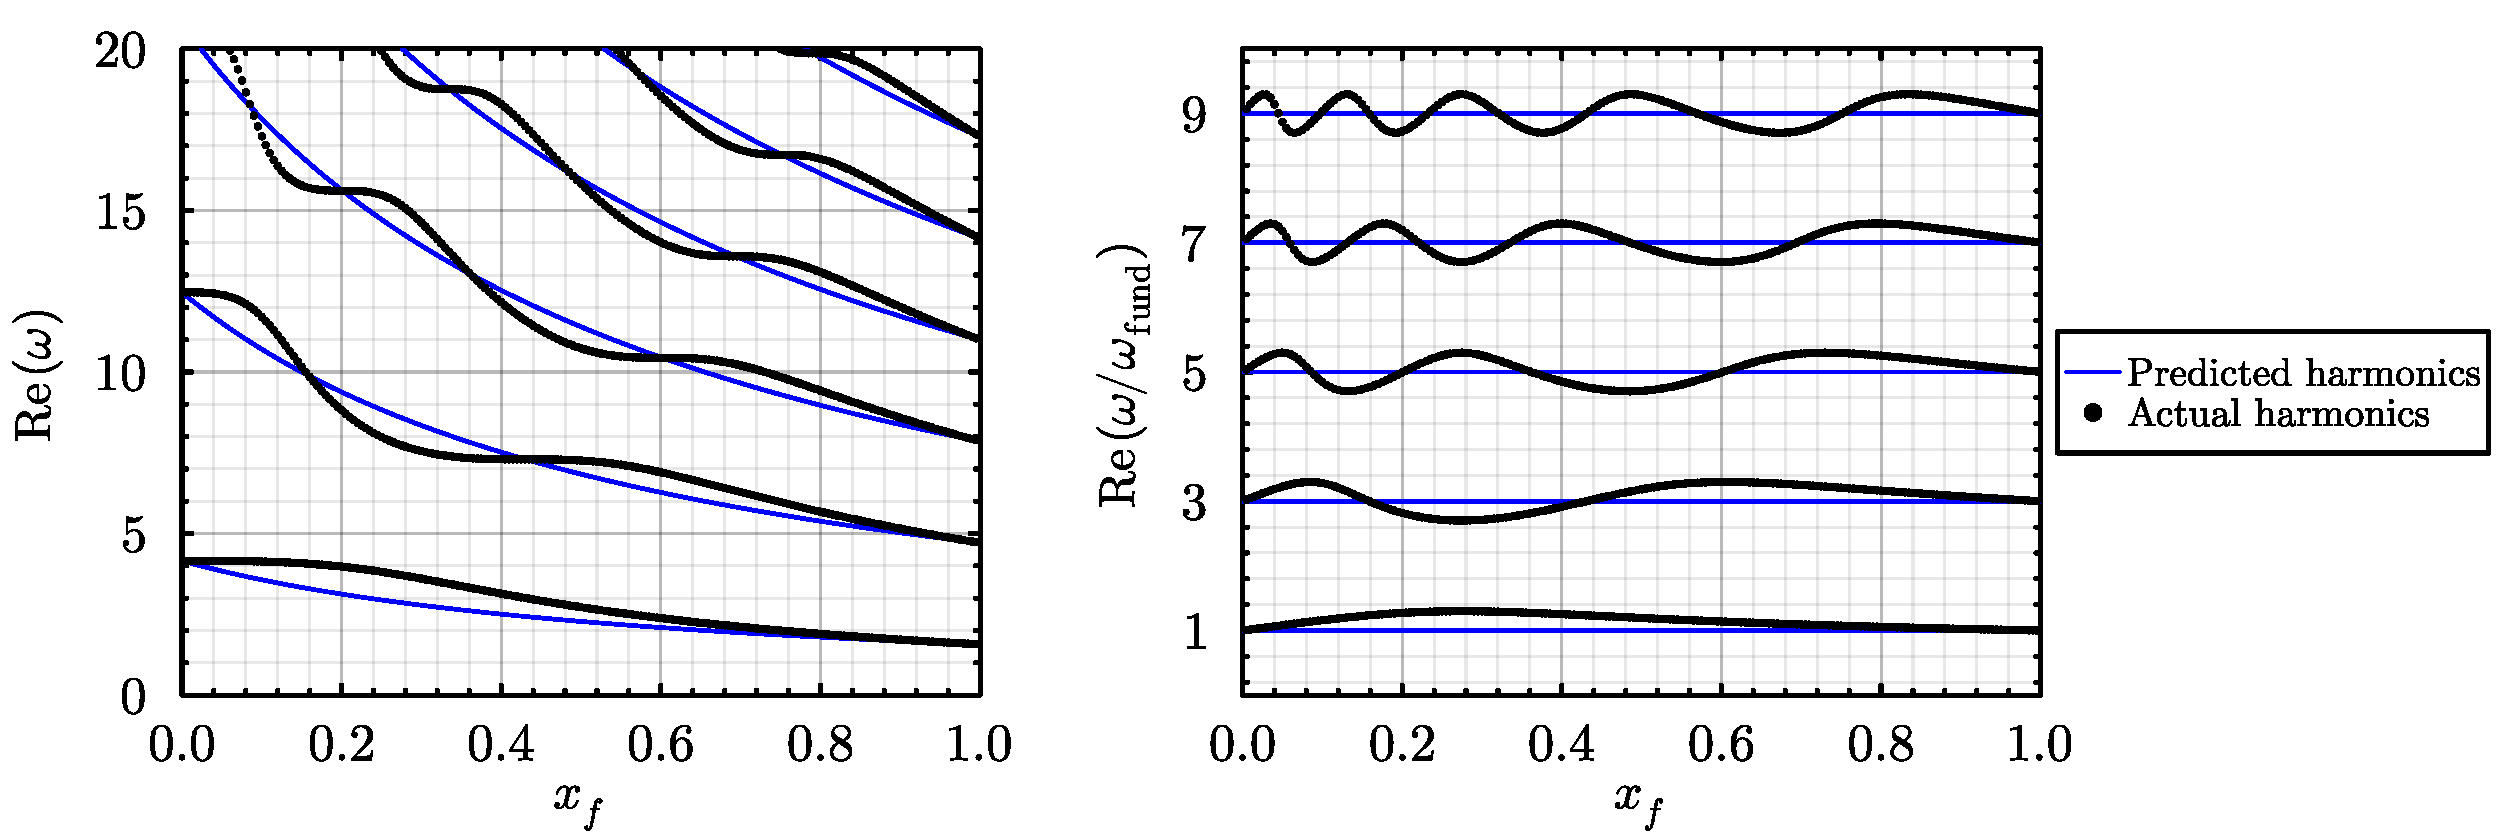
\includegraphics[scale=0.35]{assets/graphs/r=7_harmonics_both.pdf}
\caption{$r = 7$, LEFT: , RIGHT: divided by }
\label{fig:flame-harmonics}
\end{figure}

\begin{figure}[t]
\centering
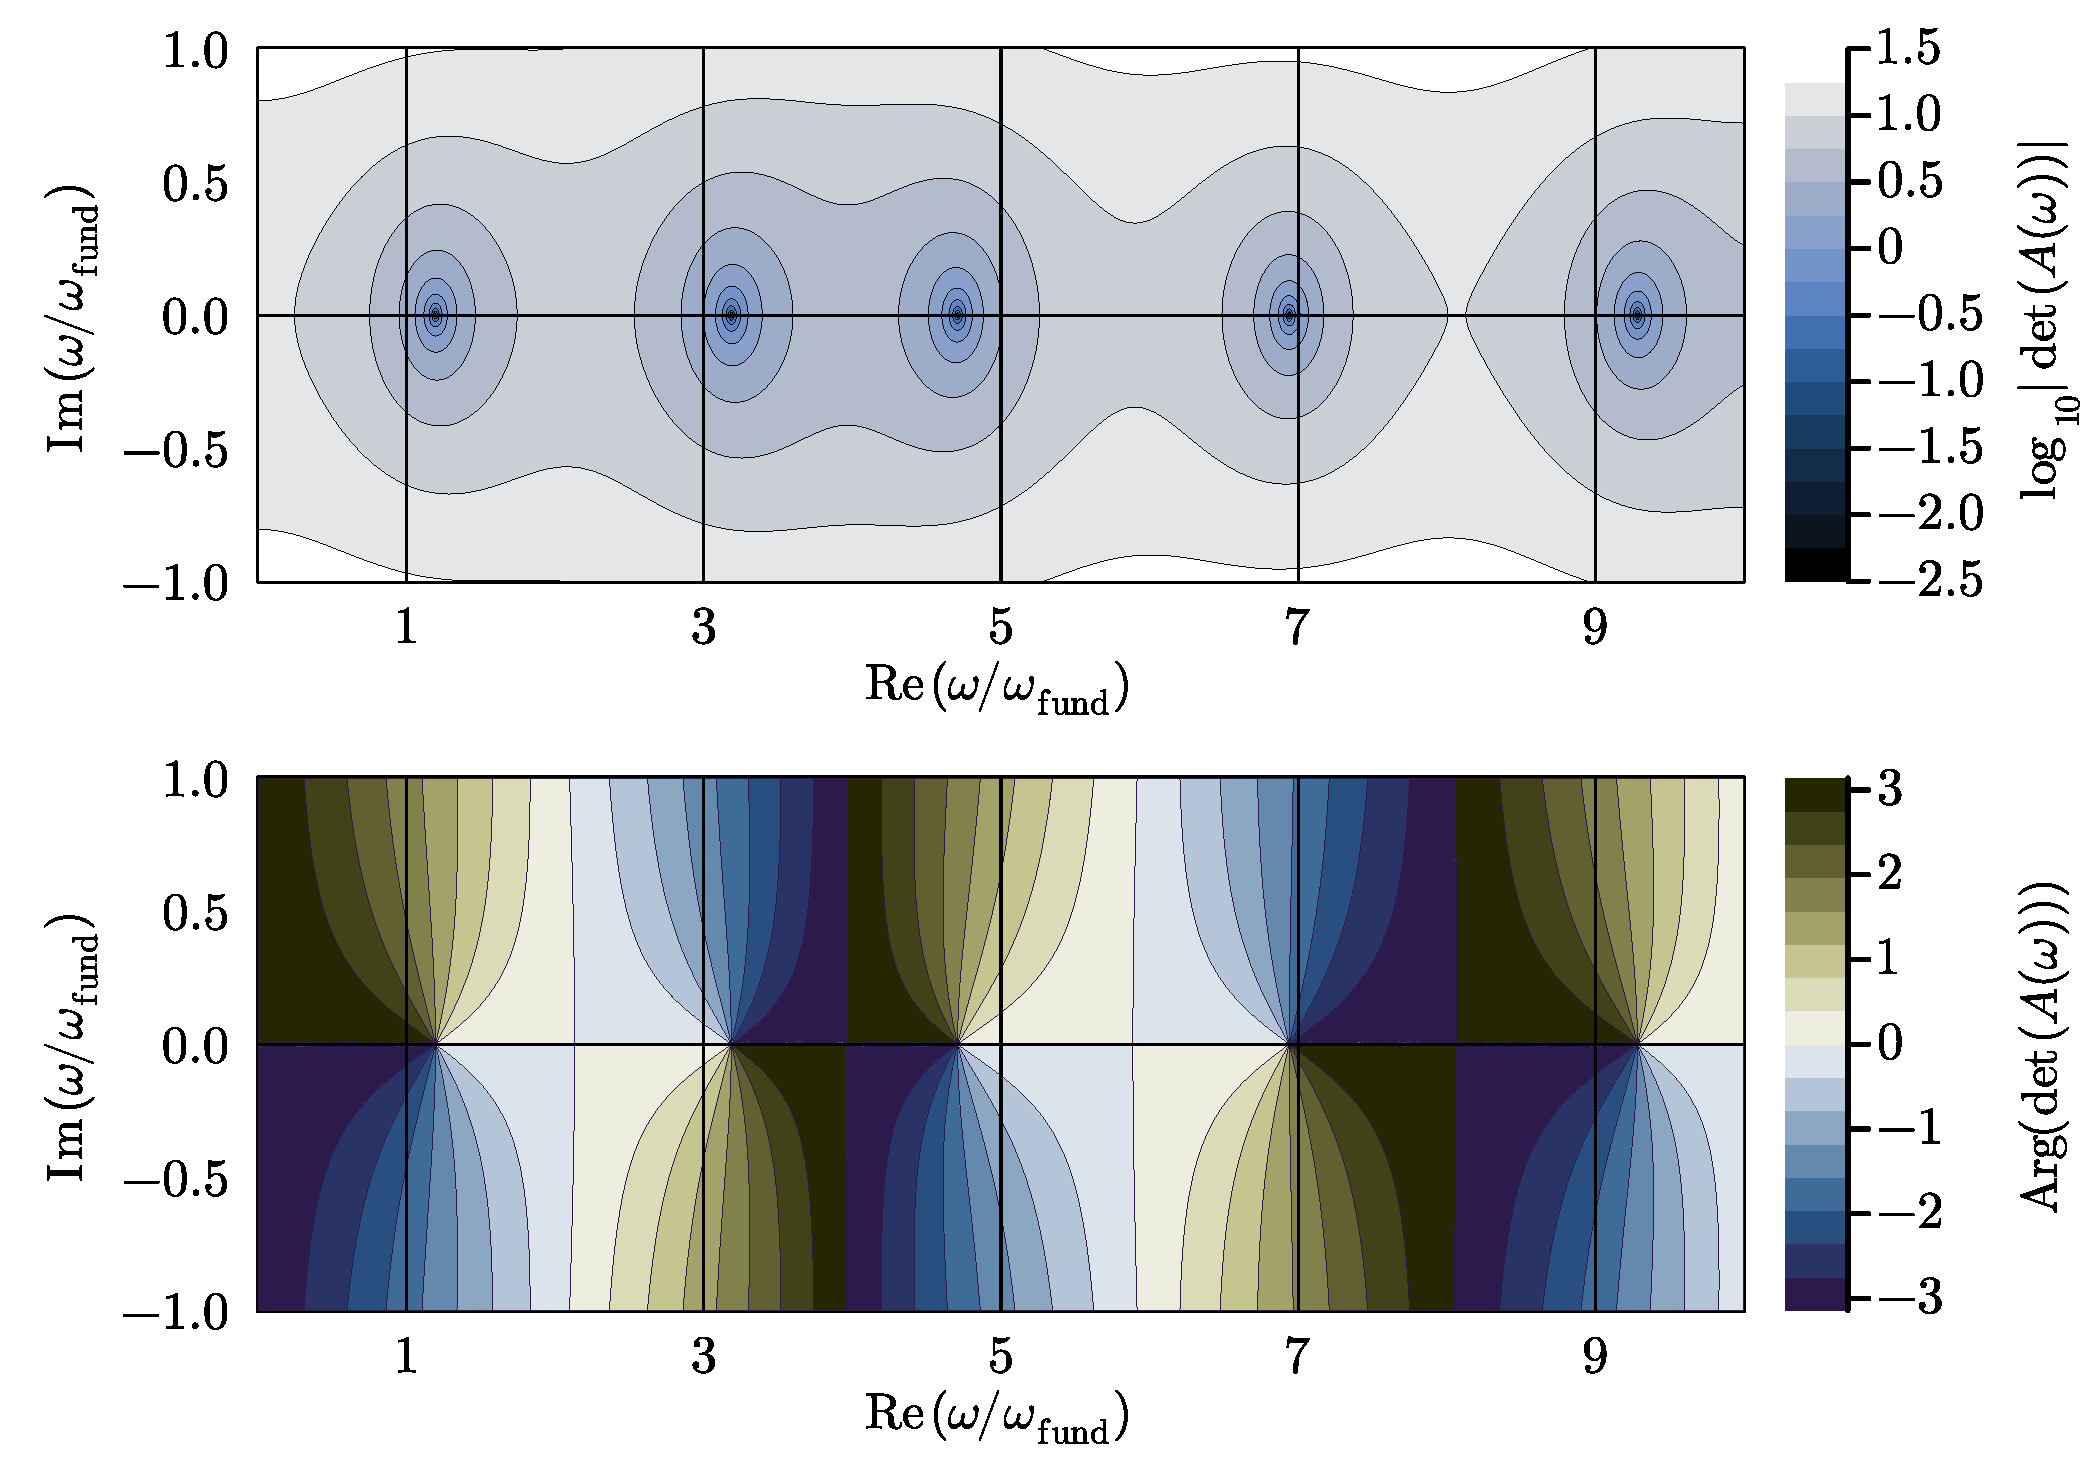
\includegraphics[scale=0.35]{assets/graphs/r=7_xf=05_complex_harmonics.pdf}
\caption{$r = 7, x_f = 0.5$, CAPTION}
\label{fig:flame-harmonics-complex}
\end{figure}

% For a flame which is .. and .., we expect harmonics of frequencies .. provided that the acoustics remain linear and are not interacting with the flame
% Note that this only accounts for the modes of a stationary density jump. If the flame is moving instead, the acoustic modes in the tube change with the moving flame. Hence the acoustics in the tube will be much more complex in this case in a way which is not predicted by this model. More complex control diagrams may be required to model the moving system instead.




\subsection{Results}

% Show some fields at an example time for both simulations

% stats data fft postprocessing/windowing

% spectrogram results

% frequencies

% mode structures!



\begin{figure}[t]
\centering
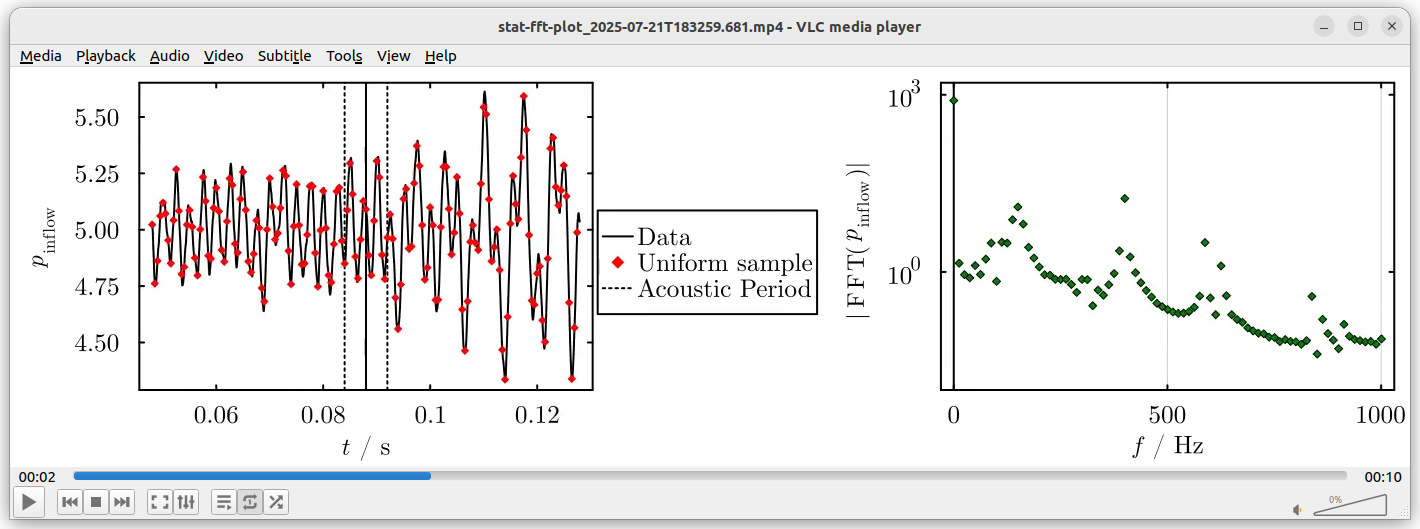
\includegraphics[scale=0.35]{assets/graphs/fft-windowing.png}
\caption{[PLACEHOLDER IMG] FFT WINDOWING}
\label{fig:windowing}
\end{figure}

\begin{figure}[t]
\centering
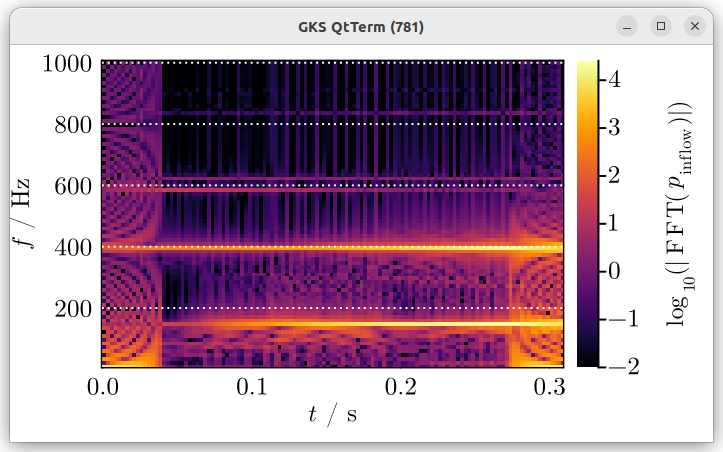
\includegraphics[scale=0.35]{assets/graphs/spectrogram.png}
\caption{[PLACEHOLDER IMG] SPECTROGRAM}
\label{fig:spectrogram}
\end{figure}

\begin{figure}[t]
\centering
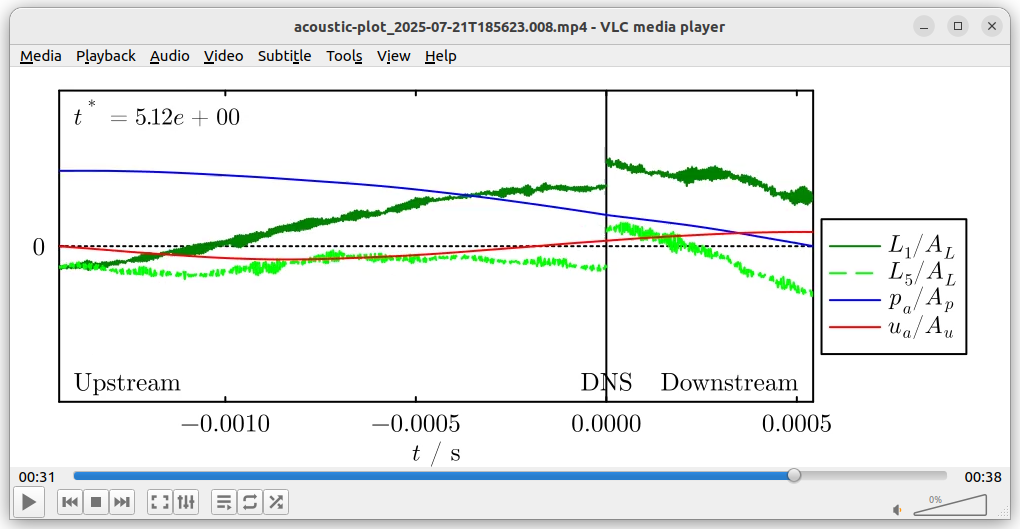
\includegraphics[scale=0.35]{assets/graphs/pp-tones.png}
\caption{[PLACEHOLDER IMG] POST-PROCESSED 1/4 AND 3/4 WAVE EVIDENCE}
\label{fig:pp-tones}
\end{figure}


